
\documentclass[border=1pt]{standalone}
\usepackage[T1]{fontenc}
\usepackage{newtxtext}
\usepackage{newtxmath}
\usepackage{amsmath}
\usepackage{tikz}
\usepackage{pgfplots}
\usepgfplotslibrary{groupplots}
\usetikzlibrary{arrows.meta}
\pgfplotsset{compat=1.18}

\definecolor{cclassical}{HTML}{2166ac}
\definecolor{clearned}{HTML}{b2182b}
\definecolor{cproposed}{HTML}{1a9850}
\definecolor{cref}{HTML}{7f7f7f}
\definecolor{clight}{HTML}{67a9cf}
\definecolor{cbandlo}{HTML}{f4a582}
\definecolor{cbandhi}{HTML}{92c5de}

% Figure text is sized for a 252 pt column: axis labels a touch under the
% 8 pt caption size, tick labels one step below that.
\newcommand{\figlab}{\fontsize{7.5}{8.5}\selectfont}
\newcommand{\figtick}{\fontsize{6.5}{7.5}\selectfont}
\newcommand{\fignote}{\fontsize{6}{7}\selectfont}

\pgfplotsset{
  every axis/.append style={
    line width=0.5pt,
    scale only axis,
    tick style={line width=0.4pt, black},
    tick pos=left,
    grid=major,
    grid style={gray!30, line width=0.3pt},
    label style={font=\figlab},
    tick label style={font=\figtick},
    title style={font=\figlab, yshift=-2pt},
    legend cell align=left,
    legend style={
      font=\fignote, draw=black!35, fill=white, fill opacity=0.92,
      text opacity=1, inner sep=1.2pt, row sep=-1.5pt, legend image post style={scale=0.7}},
  },
  every axis plot/.append style={line width=0.7pt, mark size=1.3pt},
}
\begin{document}
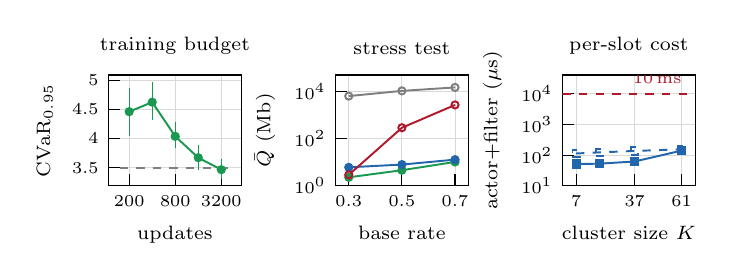
\begin{tikzpicture}
\begin{groupplot}[
  group style={group size=3 by 1, horizontal sep=34pt},
  width=48pt, height=40pt]
\nextgroupplot[title={training budget}, xmode=log, xlabel={updates}, ylabel={$\mathrm{CVaR}_{0.95}$}, xtick={200,800,3200}, xticklabels={200,800,3200}]
\addplot[cproposed, mark=*, error bars/.cd, y dir=both, y explicit,
  error bar style={line width=0.4pt}, error mark options={line width=0.4pt, mark size=1pt}]
  table[x=x, y=y, y error plus=ep, y error minus=em] {
x y ep em
200 4.46004 0.353438 0.370934
400 4.6227 0.30523 0.265807
800 4.03848 0.200741 0.156954
1600 3.67275 0.170752 0.163163
3200 3.46829 0.13912 0.118183
};

\addplot[cref, dashed, forget plot] coordinates {(150,3.5) (4200,3.5)};
\nextgroupplot[title={stress test}, ymode=log, xlabel={base rate}, ylabel={$\bar Q$ (Mb)}, xmin=0.25, xmax=0.75, xtick={0.3,0.5,0.7}, ymin=1, ymax=5e4, ytick={1e0,1e2,1e4}, yminorticks=false, legend style={at={(1.02,1.0)}, anchor=north west, draw=none, fill=none, font=\fignote}]
\addplot[cproposed, mark=*] coordinates {(0.3,2.28833) (0.5,4.5899) (0.7,10.2892)};
\addplot[cclassical, mark=*] coordinates {(0.3,6.09025) (0.5,7.96224) (0.7,12.8949)};
\addplot[clearned, mark=o] coordinates {(0.3,2.91649) (0.5,290.899) (0.7,2704.99)};
\addplot[cref, mark=o] coordinates {(0.3,6433.01) (0.5,10699.8) (0.7,14992.3)};
\nextgroupplot[title={per-slot cost}, ymode=log, xlabel={cluster size $K$}, ylabel={actor${+}$filter ($\mu$s)}, xmin=0, xmax=68, ymin=10, ymax=40000, xtick={7,37,61}, ytick={1e1,1e2,1e3,1e4}, minor tick num=0, log basis y=10, yminorticks=false]
\addplot[cclassical, mark=square*] coordinates {(7,51.086) (19,52.446) (37,61.951) (61,139.403)};
\addplot[cclassical, mark=square, dashed] coordinates {(7,112.432) (19,122.227) (37,136.172) (61,153.736)};
\addplot[clearned, dashed, forget plot] coordinates {(0,10000) (68,10000)};
\node[font=\fignote, text=clearned, anchor=south east] at (axis cs:66,10000) {10\,ms};
\end{groupplot}
\end{tikzpicture}
\end{document}
